\documentclass[conference]{IEEEtran}
\usepackage{IEEEpreamble}

\usepackage{booktabs}
\usepackage{blindtext}
\usepackage{sepnum}
\usepackage{url}
\usepackage{listings}
\usepackage{zi4}
\usepackage{minted}

\usepackage{tikz}

\lstset{
  basicstyle=\ttfamily,
}

\begin{document}
%
% paper title
% can use linebreaks \\ within to get better formatting as desired
\title{\textsc{Fuse}: A Reproducable, Internet-scale\\Dataset of Spreadsheets}

\author{
\IEEEauthorblockN{Titus Barik\IEEEauthorrefmark{1}\IEEEauthorrefmark{2}, Kevin Lubick, Justin Smith, John Slankas, Emerson Murphy-Hill}
\IEEEauthorblockA{\IEEEauthorrefmark{1}ABB Corporation Research, Raleigh, North Carolina, USA\\
North Carolina State University, Raleigh, North Carolina USA
}}

\maketitle

\begin{abstract}
We submit a corpus consisting of 1.5 million spreadsheets, extracted using the Common Crawl corpus (based on Blekko). This corpus is compared against a proprietary index from a leading search engine company to measure representative against other commercial index. This corpus is intended to replace EUSES.
\end{abstract}
% IEEEtran.cls defaults to using nonbold math in the Abstract.
% This preserves the distinction between vectors and scalars. However,
% if the conference you are submitting to favors bold math in the abstract,
% then you can use LaTeX's standard command \boldmath at the very start
% of the abstract to achieve this. Many IEEE journals/conferences frown on
% math in the abstract anyway.

% no keywords




% For peer review papers, you can put extra information on the cover
% page as needed:
% \ifCLASSOPTIONpeerreview
% \begin{center} \bfseries EDICS Category: 3-BBND \end{center}
% \fi
%
% For peerreview papers, this IEEEtran command inserts a page break and
% creates the second title. It will be ignored for other modes.
\IEEEpeerreviewmaketitle

% Oops: we forgot to handle application/vnd.oasis.opendocument.spreadsheet.

% \textbf{Data papers}. We want to encourage researchers to share their data. Data papers should describe data sets curated by their authors and made available to others. They are expected to be at most 4 pages long and should address the following: description of the data, including its source; methodology used to gather it; description of the schema used to store it, and any limitations and/or challenges of this data set. The data should be made available at the time of submission of the paper for review, but will be considered confidential until publication of the paper. Further details about data papers are available on the conference website. 

% \begin{enumerate}
% \item Description of the data.
% \item Methodology used to gather it
% \item Description of the schema used to store it
% \item Limitations and Challenges of data set
% \end{enumerate}

\section{Introduction}

\begin{minted}{js}
{
    "WARC-Record-ID": "test"
}
\end{minted}

% \begin{minted}[mathescape,
%                linenos,
%                numbersep=5pt,
%                gobble=2,
%                frame=lines,
%                framesep=2mm]{csharp}
% string title = "This is a Unicode in the sky"
% /*
% Defined as $\pi=\lim_{n\to\infty}\frac{P_n}{d}$ where $P$ is the perimeter
% of an $n$-sided regular polygon circumscribing a
% circle of diameter $d$.
% */
% const double pi = 3.1415926535
% \end{minted}

Spreadsheets are one of the most common end user programming environments~\cite{Scaffidi2005}. 
Spreadsheets provide a platform for formula-based and conditional computations. 
Within a spreadsheet, users can develop complex programs using macros. 
Like traditional programming environments, researchers have studied code smells, refactoring, and debugging in spreadsheets~\cite{Pinzger2012,Badame2012,Abraham2007}.

Such research is supported by some notable existing corpora, such as the EUSES spreadsheet corpus and the Enron spreadsheet dataset~\cite{Fisher2005}. CITE
However, the available spreadsheet corpora exhibit several limitations.
Currently spreadsheet corpora exist as snapshots; they do not provide mechanisms for reproduction or updates.
Further, with 4498 spreadsheets, the EUSES dataset represents a small sample of all existing spreadsheets and the Enron dataset contains spreadsheets from only one company.
Researchers who wish to use these corpora must manually reason about the properties of each spreadsheet as neither corpus provides spreadsheet-level metadata.
For example, a researcher only interested in studying spreadsheet macros would have to download and inspect the contents of each spreadsheet from the EUSES corpus even though only 126 contain macros.

Alternatively, we provide a corpus creation technique that overcomes many of these limitations. 
Not only is our corpus larger, but our technique is open and reproducible.  
We publicly release the scanning software used to create this corpus.
Accordingly, we encourage researchers to validate our data and methods.
Further, to help researchers navigate the dataset, we provide metadata for each spreadsheet in our corpus as well as the tool used to compute that metadata.

Columwith is: The text height is \the\columnwidth

% \begin{figure}[!t]
% \centering
% % % Created by tikzDevice version 0.8.1 on 2015-02-22 23:14:01
% !TEX encoding = UTF-8 Unicode
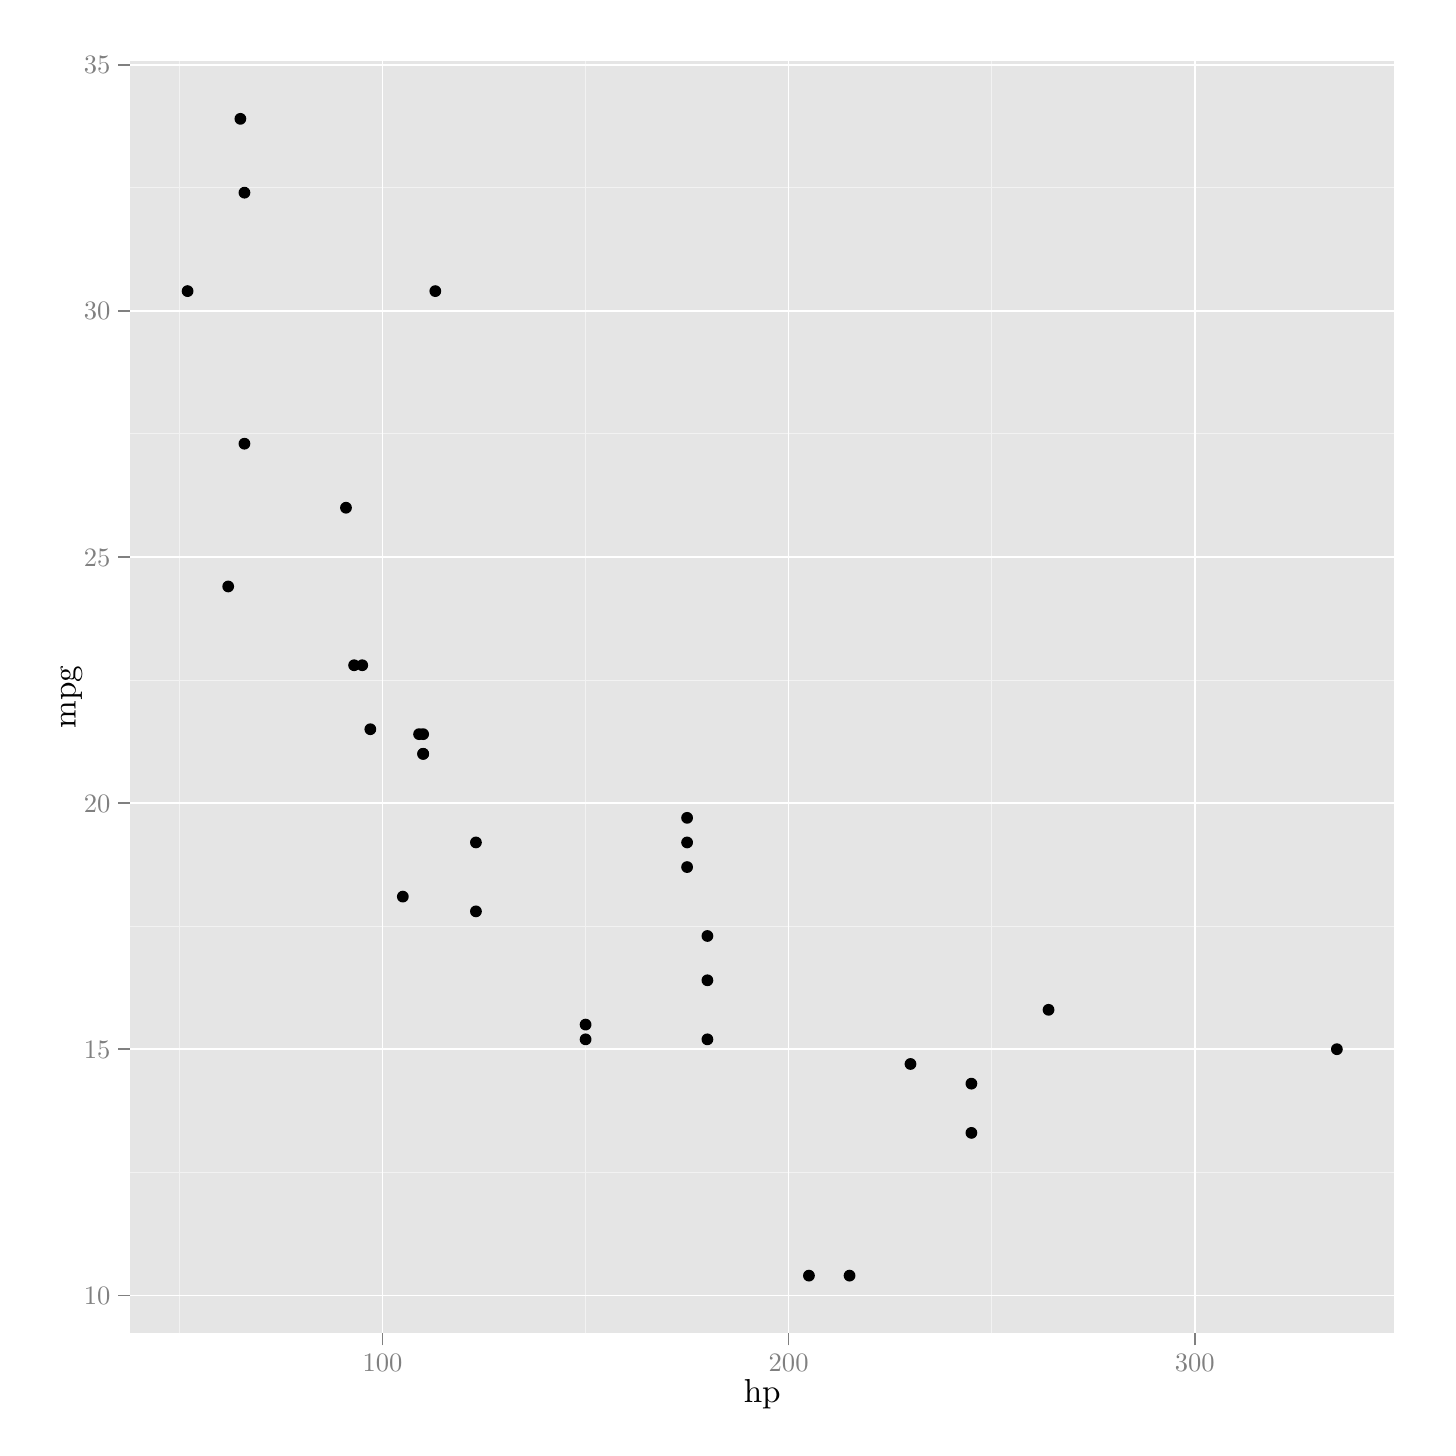
\begin{tikzpicture}[x=1pt,y=1pt]
\definecolor{fillColor}{RGB}{255,255,255}
\path[use as bounding box,fill=fillColor,fill opacity=0.00] (0,0) rectangle (505.89,505.89);
\begin{scope}
\path[clip] (  0.00,  0.00) rectangle (505.89,505.89);
\definecolor{drawColor}{RGB}{255,255,255}
\definecolor{fillColor}{RGB}{255,255,255}

\path[draw=drawColor,line width= 0.6pt,line join=round,line cap=round,fill=fillColor] (  0.00,  0.00) rectangle (505.89,505.89);
\end{scope}
\begin{scope}
\path[clip] ( 37.02, 34.03) rectangle (493.85,493.85);
\definecolor{fillColor}{gray}{0.90}

\path[fill=fillColor] ( 37.02, 34.03) rectangle (493.85,493.85);
\definecolor{drawColor}{gray}{0.95}

\path[draw=drawColor,line width= 0.3pt,line join=round] ( 37.02, 92.29) --
	(493.85, 92.29);

\path[draw=drawColor,line width= 0.3pt,line join=round] ( 37.02,181.23) --
	(493.85,181.23);

\path[draw=drawColor,line width= 0.3pt,line join=round] ( 37.02,270.17) --
	(493.85,270.17);

\path[draw=drawColor,line width= 0.3pt,line join=round] ( 37.02,359.10) --
	(493.85,359.10);

\path[draw=drawColor,line width= 0.3pt,line join=round] ( 37.02,448.04) --
	(493.85,448.04);

\path[draw=drawColor,line width= 0.3pt,line join=round] ( 54.85, 34.03) --
	( 54.85,493.85);

\path[draw=drawColor,line width= 0.3pt,line join=round] (201.60, 34.03) --
	(201.60,493.85);

\path[draw=drawColor,line width= 0.3pt,line join=round] (348.35, 34.03) --
	(348.35,493.85);
\definecolor{drawColor}{RGB}{255,255,255}

\path[draw=drawColor,line width= 0.6pt,line join=round] ( 37.02, 47.82) --
	(493.85, 47.82);

\path[draw=drawColor,line width= 0.6pt,line join=round] ( 37.02,136.76) --
	(493.85,136.76);

\path[draw=drawColor,line width= 0.6pt,line join=round] ( 37.02,225.70) --
	(493.85,225.70);

\path[draw=drawColor,line width= 0.6pt,line join=round] ( 37.02,314.63) --
	(493.85,314.63);

\path[draw=drawColor,line width= 0.6pt,line join=round] ( 37.02,403.57) --
	(493.85,403.57);

\path[draw=drawColor,line width= 0.6pt,line join=round] ( 37.02,492.51) --
	(493.85,492.51);

\path[draw=drawColor,line width= 0.6pt,line join=round] (128.22, 34.03) --
	(128.22,493.85);

\path[draw=drawColor,line width= 0.6pt,line join=round] (274.97, 34.03) --
	(274.97,493.85);

\path[draw=drawColor,line width= 0.6pt,line join=round] (421.72, 34.03) --
	(421.72,493.85);
\definecolor{fillColor}{RGB}{0,0,0}

\path[fill=fillColor] (142.90,243.48) circle (  2.13);

\path[fill=fillColor] (142.90,243.48) circle (  2.13);

\path[fill=fillColor] (117.95,275.50) circle (  2.13);

\path[fill=fillColor] (142.90,250.60) circle (  2.13);

\path[fill=fillColor] (238.28,202.57) circle (  2.13);

\path[fill=fillColor] (135.56,191.90) circle (  2.13);

\path[fill=fillColor] (341.01,124.31) circle (  2.13);

\path[fill=fillColor] ( 72.46,303.96) circle (  2.13);

\path[fill=fillColor] (120.89,275.50) circle (  2.13);

\path[fill=fillColor] (161.98,211.47) circle (  2.13);

\path[fill=fillColor] (161.98,186.56) circle (  2.13);

\path[fill=fillColor] (245.62,161.66) circle (  2.13);

\path[fill=fillColor] (245.62,177.67) circle (  2.13);

\path[fill=fillColor] (245.62,140.32) circle (  2.13);

\path[fill=fillColor] (282.31, 54.94) circle (  2.13);

\path[fill=fillColor] (296.98, 54.94) circle (  2.13);

\path[fill=fillColor] (319.00,131.42) circle (  2.13);

\path[fill=fillColor] ( 78.33,446.26) circle (  2.13);

\path[fill=fillColor] ( 57.79,410.69) circle (  2.13);

\path[fill=fillColor] ( 76.86,472.94) circle (  2.13);

\path[fill=fillColor] (123.82,252.38) circle (  2.13);

\path[fill=fillColor] (201.60,145.65) circle (  2.13);

\path[fill=fillColor] (201.60,140.32) circle (  2.13);

\path[fill=fillColor] (341.01,106.52) circle (  2.13);

\path[fill=fillColor] (238.28,211.47) circle (  2.13);

\path[fill=fillColor] ( 78.33,355.55) circle (  2.13);

\path[fill=fillColor] (115.02,332.42) circle (  2.13);

\path[fill=fillColor] (147.30,410.69) circle (  2.13);

\path[fill=fillColor] (368.89,150.99) circle (  2.13);

\path[fill=fillColor] (238.28,220.36) circle (  2.13);

\path[fill=fillColor] (473.08,136.76) circle (  2.13);

\path[fill=fillColor] (141.43,250.60) circle (  2.13);
\end{scope}
\begin{scope}
\path[clip] (  0.00,  0.00) rectangle (505.89,505.89);
\definecolor{drawColor}{gray}{0.50}

\node[text=drawColor,anchor=base east,inner sep=0pt, outer sep=0pt, scale=  0.96] at ( 29.91, 44.51) {10};

\node[text=drawColor,anchor=base east,inner sep=0pt, outer sep=0pt, scale=  0.96] at ( 29.91,133.45) {15};

\node[text=drawColor,anchor=base east,inner sep=0pt, outer sep=0pt, scale=  0.96] at ( 29.91,222.39) {20};

\node[text=drawColor,anchor=base east,inner sep=0pt, outer sep=0pt, scale=  0.96] at ( 29.91,311.33) {25};

\node[text=drawColor,anchor=base east,inner sep=0pt, outer sep=0pt, scale=  0.96] at ( 29.91,400.27) {30};

\node[text=drawColor,anchor=base east,inner sep=0pt, outer sep=0pt, scale=  0.96] at ( 29.91,489.21) {35};
\end{scope}
\begin{scope}
\path[clip] (  0.00,  0.00) rectangle (505.89,505.89);
\definecolor{drawColor}{gray}{0.50}

\path[draw=drawColor,line width= 0.6pt,line join=round] ( 32.75, 47.82) --
	( 37.02, 47.82);

\path[draw=drawColor,line width= 0.6pt,line join=round] ( 32.75,136.76) --
	( 37.02,136.76);

\path[draw=drawColor,line width= 0.6pt,line join=round] ( 32.75,225.70) --
	( 37.02,225.70);

\path[draw=drawColor,line width= 0.6pt,line join=round] ( 32.75,314.63) --
	( 37.02,314.63);

\path[draw=drawColor,line width= 0.6pt,line join=round] ( 32.75,403.57) --
	( 37.02,403.57);

\path[draw=drawColor,line width= 0.6pt,line join=round] ( 32.75,492.51) --
	( 37.02,492.51);
\end{scope}
\begin{scope}
\path[clip] (  0.00,  0.00) rectangle (505.89,505.89);
\definecolor{drawColor}{gray}{0.50}

\path[draw=drawColor,line width= 0.6pt,line join=round] (128.22, 29.77) --
	(128.22, 34.03);

\path[draw=drawColor,line width= 0.6pt,line join=round] (274.97, 29.77) --
	(274.97, 34.03);

\path[draw=drawColor,line width= 0.6pt,line join=round] (421.72, 29.77) --
	(421.72, 34.03);
\end{scope}
\begin{scope}
\path[clip] (  0.00,  0.00) rectangle (505.89,505.89);
\definecolor{drawColor}{gray}{0.50}

\node[text=drawColor,anchor=base,inner sep=0pt, outer sep=0pt, scale=  0.96] at (128.22, 20.31) {100};

\node[text=drawColor,anchor=base,inner sep=0pt, outer sep=0pt, scale=  0.96] at (274.97, 20.31) {200};

\node[text=drawColor,anchor=base,inner sep=0pt, outer sep=0pt, scale=  0.96] at (421.72, 20.31) {300};
\end{scope}
\begin{scope}
\path[clip] (  0.00,  0.00) rectangle (505.89,505.89);
\definecolor{drawColor}{RGB}{0,0,0}

\node[text=drawColor,anchor=base,inner sep=0pt, outer sep=0pt, scale=  1.20] at (265.43,  9.03) {hp};
\end{scope}
\begin{scope}
\path[clip] (  0.00,  0.00) rectangle (505.89,505.89);
\definecolor{drawColor}{RGB}{0,0,0}

\node[text=drawColor,rotate= 90.00,anchor=base,inner sep=0pt, outer sep=0pt, scale=  1.20] at ( 17.30,263.94) {mpg};
\end{scope}
\end{tikzpicture}

% \caption{Test plot.}
% \label{fig:testplot}
% \end{figure}

Our contributions are 
\begin{enumerate}
\item A corpus of ??? spreadsheets pulled from the pubic web
\item A pipeline of tools that allows other researchers to more easily perform spreadsheet extraction and analysis at scale
\item A detailed set of metadata for this corpus and two other corpora [foo], [bar]  which allow researchers to make queries without having to download or analyze the entire spreadsheet corpus.  
\end{enumerate}

% \begin{figure}[!t]
% \centering
% \includegraphics[width=\columnwidth]{corpora}
% \caption{Comparison matrix of available spreadsheet corpora. How does \textsc{Fuse} stack up?}
% \label{fig:corpora}
% \end{figure}

\begin{figure*}[!t]
\centering
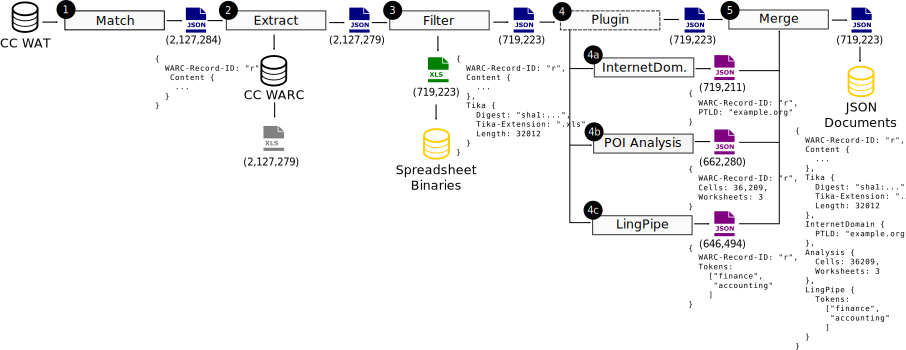
\includegraphics[width=\linewidth]{pipeline}
\caption{The MapReduce pipeline for extracting spreadsheets and associated spreadsheet metadata from Common Crawl. In \textsc{Crawl} (Stage 1), WAT segments containing HTTP headers and offset information into WARC records are parsed. Records that heuristically match spreadsheets (e.g., a \texttt{Content-Type} of \texttt{application/vnd.ms-excel} are retained. In \textsc{Extract} (Stage 2), ...}
\label{fig:mrpipeline}
\end{figure*}

% Improve display of JSON files
% http://tex.aspcode.net/view/635399273629833626148902/how-to-improve-listings-display-of-json-files

% TODO(tbarik)
%  This WAT file is okay, but the corresponding WARC record is corrupt:
% Put an example of this issue in the methodology.
%  {"WARC-Date":"2014-09-22T12:11:35Z","WARC-Record-ID":"<urn:uuid:0d670ac1-319f-42b0-89bf-7c52dd51e1dd>","Content-Length":1385,"WARC-Target-URI":"http://www.medcom.dk/dwn1514.xls","WARC-Content-Type":"application/json","Content":{"Envelope":{"Format":"WARC","WARC-Header-Length":"350","Block-Digest":"sha1:6JCTYB2KGCZ5YX63EFLECRMXB4KUBOQB","Actual-Content-Length":"263","WARC-Header-Metadata":{"WARC-Type":"request","WARC-Date":"2014-09-22T12:11:35Z","WARC-Warcinfo-ID":"<urn:uuid:1c4997f8-bc87-4ade-8efd-47f4cb8ce2a6>","Content-Length":"263","WARC-Record-ID":"<urn:uuid:81815bbd-d47d-4755-8e41-d820a1d05043>","WARC-Target-URI":"http://www.medcom.dk/dwn1514.xls","WARC-IP-Address":"91.193.139.41","Content-Type":"application/http; msgtype=request"},"Payload-Metadata":{"Trailing-Slop-Length":"4","HTTP-Request-Metadata":{"Headers":{"Accept-Language":"en-us,en-gb,en;q=0.7,*;q=0.3","Host":"www.medcom.dk","Accept-Encoding":"x-gzip, gzip, deflate","User-Agent":"CCBot/2.0 (http://commoncrawl.org/faq/)","Accept":"text/html,application/xhtml+xml,application/xml;q=0.9,*/*;q=0.8"},"Headers-Length":"261","Entity-Length":"0","Entity-Trailing-Slop-Bytes":"0","Request-Message":{"Method":"GET","Version":"HTTP/1.0","Path":"/dwn1514.xls"},"Entity-Digest":"sha1:3I42H3S6NNFQ2MSVX7XZKYAYSCX5QBYJ"},"Actual-Content-Type":"application/http; msgtype=request"}},"Container":{"Compressed":true,"Gzip-Metadata":{"Footer-Length":"8","Deflate-Length":"418","Header-Length":"10","Inflated-CRC":"505390695","Inflated-Length":"617"},"Offset":"654053188","Filename":"CC-MAIN-20140914011217-00240-ip-10-234-18-248.ec2.internal.warc.gz"}},"WARC-Refers-To":"<urn:uuid:81815bbd-d47d-4755-8e41-d820a1d05043>","Path":"common-crawl/crawl-data/CC-MAIN-2014-41/segments/1410657137046.16/wat/CC-MAIN-20140914011217-00240-ip-10-234-18-248.ec2.internal.warc.wat.gz"}


similar in size to other large corpora
representativeness against Google index
metadata

helps with tool evaluation

accessible -- getting this for yourself is a high cost maybe 5k

this set is reproducable
compared with existing data sets, it is new -- the others are more than a decade old.

even the enron corpus is 15000 spreadsheets -- whoopee. But it's good to compare against since it's a private corpus.

The contribution of this paper is:

\begin{itemize}
\item Foo
\end{itemize}

go to figshare
% http://figshare.com/articles/Enron_s_Spreadsheets_and_Related_Emails_A_Dataset_and_Analysis/1222882


what metrics?

happy medium between euses and google

deliberate design decision to 
intentionally spluit the data into metadata and binary phases

\section{Methodology}

\begin{table}[!t]
\caption{Common Crawl Archive\label{tab:ccrawl}}
\centering
\begin{tabular}{lll}
\toprule
Description & TB & Yield\\
\midrule
Summer 2013 & 30.6 & 42.14\%\\
Winter 2013 & 35.1 & 33.46\% \\
March 2014 & 36.4 & \\
April 2014 & 41.2 & \\
July 2014 & 59.2 & \\
August 2014 & 46.6 & \\
September 2014 & 48.9 & \\
October 2014 & 59.1 & \\
November 2014 & 31.4 & \\
December 2014 & 35.2 & \\
\bottomrule
\end{tabular}
\end{table}


We selected the Common Crawl\footnote{\url{http://commoncrawl.org}} index as the primary source for our spreadsheet corpus, because it contains over ???TB of publicly available web crawl data and is regularly updated.

To extract spreadsheets from this index, first we crawled all the available WAT files in the index targeting files that could potentially be spreadsheets, including files tagged with MSDN content types, and files with extensions containing ``.xls''. 
This crawl was the most computationally intensive task in our pipeline, consuming approximately ??? hours of CPU time. 
The crawl identified ??? candidate spreadsheets which we extracted from their associated WARC files. 

Because the WAT files contained some incomplete and incorrect tags, we extracted some invalid spreadsheets in the first phase. We used Tika\footnote{\url{http://tika.apache.org}} to identify the valid spreadsheets and then filtered out the invalid files. This stage resulted in ??? valid spreadsheets.
 
Next we processed the valid spreadsheets using Apache POI\footnote{\url{http://poi.apache.org}} to extract metadata from each spreadsheet (see Section \ref{sec:schema}). By computing a sha512 hash we identified and removed duplicate spreadsheets, resulting in a final total of ??? spreadsheets. 

+ TODO(tbarik): Copy Mixin and JsonMerge, not shown, but utility tool to easily copy sets and merge them.

\subsection{MapReduce Pipeline}

\subsubsection{Crawl} 

In this step, 

\subsubsection{Extract} 

In this step,

\subsubsection{Filter} 

In this step,
\subsubsection{Mixin} 

In this step,

\subsubsection{Merge} 

In this step,

% https://publicsuffix.org/list/

% sebastien paper for other metrics a look inside common crawl
% http://blog.commoncrawl.org/2013/08/a-look-inside-common-crawls-210tb-2012-web-corpus/
% domain parsing is done using 

% https://publicsuffix.org/

limitation: truncation, 2 MB, 5 MB?

% http://www.statmethods.net/advgraphs/images/ggplotdensity.png

+ TODO(tbarik): Stages or tasks?

needed to create WAT index files

% dremel> select COUNT(doc.DocId) FROM docjoin.base WHERE doc.content.ContentType = 23;
% +------------------+
% | COUNT(doc.DocId) |
% +------------------+
% |          1635142 |
% +------------------+
% WARNING: Partition skipped
% WARNING: ~0.0% of data was not scanned (see "settings min_completion_ratio")
% 1 row in result set (319.28 sec)
% Scan rate: 37.38M rows/sec, SWE cost: 7.28138s

% dremel> select doc.DocId, RIGHT(doc.URL, 30), doc.Pagerank FROM docjoin.base WHERE doc.content.ContentType = 23 L
% IMIT 20;
% +----------------------+--------------------------------+--------------+
% | doc.DocId            | RIGHT(doc.URL, 30)             | doc.Pagerank |
% +----------------------+--------------------------------+--------------+
% | 18262361551973990081 | Noticias/210111pssufal2011.xls |        45696 |
% | 18262514318872388335 | E7%99%BB%E8%AE%B0%E8%A1%A8.xls |        53441 |
% | 18262628117481929248 | ameck-cd57ffgym.fr/file/31037/ |        49536 |
% | 18262462250520031836 | uation%20risque%20chimique.xls |            1 |
% | 18262515209375261799 | 9206/file/4%20LISTE%202014.xls |        51664 |
% | 18262601711327171729 | d_org=200054&id_dokumenty=1069 |        51318 |
% | 18262429851281169486 | loads/2009/11/distributori.xls |        47265 |
% | 18262677137761586621 | /03_Zahlungen_Schulversion.xls |        49376 |
% | 18262497829673811111 | FULL_SCHOOL_LIST_1982-1983.xls |        55771 |
% | 18098709049136093897 | 1_Guelleberechnungstabelle.XLS |        48219 |
% | 18098336056523698774 | 46658c58776252a270492189fd.xls |        51278 |
% | 18098420930462689378 | 2nd_and_3rd_Posting)_FINAL.xls |        46743 |
% | 18221693724751189184 | /stories/papka_bossa/rosta.xls |            1 |
% | 18221288433906859741 | mediaprodukciyu-22.12.2013.xls |        45065 |
% | 18221490419625251728 | 75817255013/files/sadowara.xls |        52813 |
% | 18221566511153360853 | ostnica-arhitektura_plosca.xls |        49301 |
% | 18221440248932413652 | 83%D1%81%D0%BA%D0%B8%D0%B9.xls |        44383 |
% | 18221602484570358598 | ents/0000000/44/25ichiran5.xls |        52927 |
% | 18221337705568163749 | es/201011/2010111710570042.xls |        52262 |
% | 18221462757268787142 | 20%D0%AF%D0%9D%D0%90%D0%9E.xls |        49763 |
% +----------------------+--------------------------------+--------------+
% 20 rows in result set (26.13 sec)
% Scan rate: 0.04M rows/sec, SWE cost: 6.4e-05s

For Summer 2013, Winter 2013, and March 2013, no pre-created WAT path files were available. To manually create this we did:



% aws s3 ls --recursive s3://aws-publicdatasets/common-crawl/crawl-data/CC-MAIN-2014-10/segments | awk '$4 ~ /wat/ {print $4}' > wat.summer2013.path

how did we decide to filter? MSDN content-type

% http://blogs.msdn.com/b/vsofficedeveloper/archive/2008/05/08/office-2007-open-xml-mime-types.aspx

google obtained from proprietary database query that extracted from google index all spreadsheets with content type application/ms-excel.

common crawl
segments -> subproblems

docjoiner

\emph{cleaning}

put lingpipe
put interndomain
put analysistool

\section{Description of Spreadsheet Corpus}

% What domains are represented in the corpus?

\begin{lstlisting}
db.s.aggregate(
    { "$project": 
      {"InternetDomainName.Public-Suffix" : true } },
    { "$group": 
      {"_id": "$InternetDomainName.Public-Suffix", "count": {"$sum": 1} } },
    { "$sort": { "count" : -1 } },
    { "$limit": 10 }
)
\end{lstlisting}

% TLD bias: http://w3techs.com/technologies/overview/top_level_domain/all

since it's sdescription of corpus, should be descriptive?
counts avg etc.

absfrequency, relativefrequency
gov, 250211
org, 171845
com, 112573
edu, 63572
gov.au, 43490
pa.us, 7621
net, 7409
mn.us, 4641
ac.uk, 3423
ca.us, 3003

% FOR SDL: topleveldomain

absfreq, relfreq
census.gov, 143135
triathlon.org, 106486
amamanualofstyle.com, 45118
abs.gov.au, 42941
utah.gov, 22242
ohio.gov, 16739
usda.gov, 13016
worldbank.org, 11062
theahl.com, 10350
eia.gov, 8216

\noindent\textbf{RQ: How many domains are represented?}

4,381 domains. After dedup, 4,342.

RQ what types of headers do people use?


how canonical are urls?

not very

% db.s.aggregate(
%     { "$project": {"Tika.Digest": true, "WARC-Target-URI": true } },
%     { "$group": { "_id": { uri: "$WARC-Target-URI", sha: "$Tika.Digest" }, count: { "$sum": 1 } } },    
%     { "$group": { "_id": { uri: "$_id.uri" }, count: { "$sum": 1 } } },
%     { "$match": { "count" : { "$gte" : 2 } } },
%     { "$sort": { "count" : -1 } }  
% )




results from this can be used to guide future crawls to increase the diversity of the spreadsheet corpus.

% euses and cc overlap
% sha1:24af0f8d6a5a18a44150a6b56587582546a0ba71  (1)
%   Inventory control form www.edu.edu
%    ./inventory/processed/InventoryControlForm.xls
% sha1:70cc5c391b4e439c61e003f0c01ea573fcea544b (3/but all same)
%     ncdenr.org
%     ./modeling/processed/labrates050104.xls
% sha1:9992cd834d4824cbb05c26b0ffcecff04509334c
%     naaccr.org
%     ./grades/processed/naaccr9a.xls
% sha1:9a09b5a28eb4faf6516ddac8aaf7c90eddc47090
%     http://www.courts.delaware.gov/forms/download.aspx?ID=21098
%     http://www.courts.delaware.gov/forms/download.aspx?id=21098
%     ./financial/processed/finanacial%20sheet.xls
% sha1:d903ce9171061b482d92aa78bb2e60404ab16732
%     nigc.gov
%     ./inventory/processed/TableInventorySlipWorksheet.xls    

% Media Type

Actually looking at binaries, so this looks at dedup:

application/vnd.ms-excel, 238673
application/vnd.openxmlformats-officedocument.spreadsheetml.sheet, 10555
application/vnd.openxmlformats-officedocument.spreadsheetml.template, 148

all zero:
application/vnd.ms-excel.sheet.macroEnabled.12
application/vnd.ms-excel.template.macroEnabled.12
application/vnd.ms-excel.addin.macroEnabled.12
application/vnd.ms-excel.sheet.binary.macroEnabled.12

RQ: How much can you trust HTTP headers?

RQ: Train a text classifier to identify topicality.

RQ: Evolution of spreadsheets



Breakdown of analysis:
%db.spreadsheet.aggregate(
%    { "$project": 
%      {"Summary.errorNotification" : true } },
%    { "$group": 
%      {"_id": "$Summary.errorNotification", "count": {"$sum": 1} } },
%    { "$sort": { "count" : -1 } },
%    { "$limit": 10 })

"OK", 112421
"CORRUPT",87574
"OTHER", 31676 
"BIFF5",  17643 
"ENCRYPTED",  62 



% some ideas for things to show
% http://blog.commoncrawl.org/2012/05/


place a non-shitty graph here

% http://www.felienne.com/archives/3634
\begin{table}[!t]
%% increase table row spacing, adjust to taste
%\renewcommand{\arraystretch}{1.3}
% if using array.sty, it might be a good idea to tweak the value of
% \extrarowheight as needed to properly center the text within the cells
\caption{Comparison of \textsc{Fuse} and other spreadsheet corpora\label{tab:corpora}}
\centering
%% Some packages, such as MDW tools, offer better commands for making tables
%% than the plain LaTeX2e tabular which is used here.
\begin{tabular}{lllll}
\toprule
& \textbf{\textsc{Fuse}} & \textbf{EUSES} & \textbf{Enron}\\
\midrule
Size ($n$) & 249,376 & 6,000 & 15,570\\
Space (GB) & b & 0.64 & 23.3\\
Research access & All & Researchers & All\\
Unique formulas & 894361 & 693266 & 84004\\
Extendable & Yes & Not scalable & No\\
Framework & Hadoop & Excel + VBA & Scantool\\
TIme Period & 2006 & 2006 & 2006\\
\bottomrule
\end{tabular}
\end{table}

A summary of your spreadsheet corpus can be found in Table~\ref{tab:corpora}.

\section{Results}

\subsection{Classification of spreadsheets}


\begin{table}[!t]
\caption{Spreadsheet Classification\label{tab:ccrawl}}
\centering
\begin{tabular}{lll}
\toprule
\textbf{Category} & \textbf{\textsc{Fuse}} & \textbf{EUSES}\\
\midrule
Database & 4518 & 720\\
Finance & 3058 & 780\\
Grade & 2915 & 731\\
Homework & 61 & 682\\
Inventory & 2243 & 756\\
Model & 2143 & 966\\
\bottomrule
\end{tabular}
\end{table}

The results in this section are intended to demonstrate the essential properties of the corpus.

\subsection{RQ2: How diverse is the common common crawl corpus?}
\subsection{RQ1: How stable are URIs?}
\subsection{RQ3: NLP Extraction of Spreadsheet?}
\subsection{RQ4: What types of formulas ar eused by end-user software programmers?}


Top two formulas are the same across the three corpora: 
1. Add up the three cells to my left
2. Add up the two cells to my left
And most of the top 10 are Add up n cells to my left.
Fuse \#3 HYPERLINK("http://www.eia.doe.gov/totalenergy/data/monthly/dataunits.cfm","Note: Information about data precision and revisions.")
Enron \#3 NOW()  

give warc record ids

% stage 1 metadata

\section{Data Schema}
\label{sec:schema}
In this section, we describe the schema.
The metadata we collected for the indices was largely influenced by the summary statistics presented in \cite{Fisher2005}.  
For each spreadsheet, there are over 450 entries, so we will not list them all here.
In general, the entries summarize the contents of the cells.
To list a few examples, the number of times a given Excel function (such as SUM or VLOOKUP) is used, the total number of input or data cells, the number of numeric input cells, the number of formulas used more than 50 times, the most common formula used, etc.


render json

\begin{lstlisting}
asdfsdf
\end{lstlisting}

\section{Mixins}

how do you get it?

csv file
mongodb recordobject warc extracts


% TODO(tbarik): Switch this table.


\section{Dataset Challenges and Limitations}

% https://gist.github.com/anonymous/8373f8a08a357146c20b

% https://groups.google.com/forum/#!topic/common-crawl/MV5yYWPWC_M
% As Kevin said, you might be able to get away using off the shelf search APIs, depending on exactly how much you want. One thing I will note though is that a MapReduce job over the relevant text data of Common Crawl won't cost hundreds of dollars, it would more likely cost somewhere between $30 and $60, possibly far cheaper if you run particularly optimized code.

% To combine all of them explicitly would just result in duplication of stored files, which is quite an issue when we're talking hundreds of terabytes.

% As all the files are stored in ARC or WARC, both web archive formats, the easiest way to combine them for your "full crawl" is to simply enumerate over all the files in all the crawls. This also allows you to decide what behaviour you would like (i.e. keep all pages, keep only the most recent pages, etc).

% https://groups.google.com/forum/#!topic/common-crawl/wb3jXh8x8Tg
% There are far more than 4.05 billion new web pages in the last three months. These crawls shouldn't be considered representative of how much of the web has changed or been updated in a given period of time as we only crawl a relatively small portion of the web. It also strongly depends on your definition of new, though that's a large and complicated situation all to itself.

relevance is dependent on common crawl definition of relevant

\section{Conclusion}
The conclusion goes here.

\section{Related Work}

% http://link.springer.com/article/10.1007/s10664-011-9181-9

\subsection{Why use spreadsheets}

\cite{Chambers2010} Use spreadsheet corpus + interviews to determine which features end-users use.

~\cite{Pinzger2012} Detecting code smells in spreadsheets. Analyze EUSES to study occurrence of smells.

~\cite{Badame2012} Refactor spreadsheet formula. Perform case study using EUSES dataset.

~\cite{Abraham2007} Support debugging spreadsheets

\subsection{What other corpora?}
EUSES~\cite{Fisher2005}

~\cite{Chen2013} Automatically extract relational data from spreadsheets. Extracted 410,554 spreadsheets from clue09 web crawl.

ENRON find citation <-- icse seip 2015

~\cite{Chen2013} Automatically extract relational data from spreadsheets. Extracted 410,554 spreadsheets from clue09 web crawl.


\textbf{Existing corpora.}
\textbf{Spreadsheet tools.}



% conference papers do not normally have an appendix


% use section* for acknowledgement
\section*{Acknowledgment}

This material is based upon work supported in whole or in part with funding from the Laboratory for Analytic Sciences (LAS). Any opinions, findings, conclusions, or recommendations expressed in this material are those of the author(s) and do not necessarily reflect the views of the LAS and/or any agency or entity of the United States Government.

Just kidding, I did this all by myself.

% trigger a \newpage just before the given reference
% number - used to balance the columns on the last page
% adjust value as needed - may need to be readjusted if
% the document is modified later
%\IEEEtriggeratref{8}
% The "triggered" command can be changed if desired:
%\IEEEtriggercmd{\enlargethispage{-5in}}

% references section

\raggedright
% can use a bibliography generated by BibTeX as a .bbl file
% BibTeX documentation can be easily obtained at:
% http://www.ctan.org/tex-archive/biblio/bibtex/contrib/doc/
% The IEEEtran BibTeX style support page is at:
% http://www.michaelshell.org/tex/ieeetran/bibtex/
\bibliographystyle{IEEEtran}
% argument is your BibTeX string definitions and bibliography database(s)
\bibliography{library}


% that's all folks
\end{document}


